\documentclass[a4paper]{article}
\usepackage[a4paper]{geometry}
\usepackage{amsmath}
\usepackage{amssymb}
\usepackage[utf8]{inputenc}
\usepackage{graphicx}
\usepackage{booktabs}
\usepackage[russian]{babel}

\title{Лабораторная работа 2.3.1 \\Получение и измерение вакуума}
\date{19 февраля 2017 г.}
\author{Вячеслав Ждановский, студент 611 группы ФРКТ\\
Шамиль Вагабов, студент 611 группы ФРКТ\\
Станислав Токарев, студент 611 группы ФРКТ}

\begin{document}
	\pagenumbering{gobble}
	\maketitle
	\newpage
	\pagenumbering{arabic}
	\paragraph{Цель работы:}
	измерение объёмов форвакуумной и высоковакуумной частей устновки; определение скорости откачки системы в стационарном режиме, а также по ухудшению и по улучшению вакуума.
	\paragraph{В работе используются:}
	вакуумная установка с манометрами: масляным, термопарным и ионизационным.
	\section{Схема экспериментальной установки}
	\begin{figure}[h!]
		\centering
		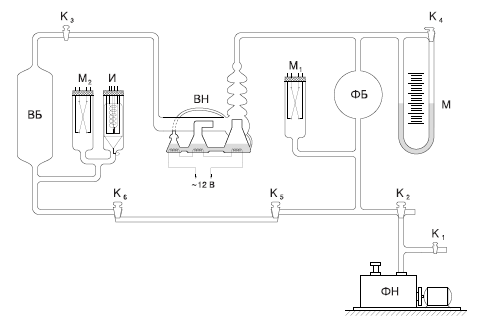
\includegraphics[width=90mm]{pic.png}
		\caption{Схема экспериментальной установки \label{overflow}}
	\end{figure}
	\begin{figure}[h!]
		\centering
		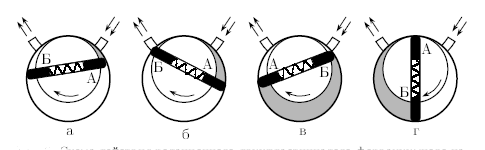
\includegraphics[width=90mm]{pic1.png}
		\caption{Схема действия ротационного двухпластинчатого форвакуумного насоса\label{overflow}}
	\end{figure}
	\begin{figure}[h!]
		\centering
		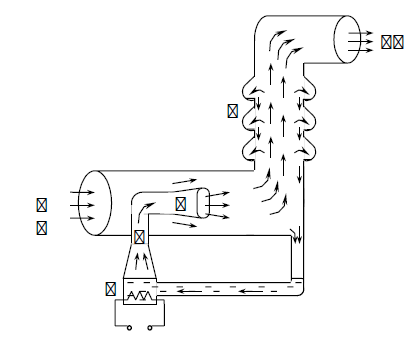
\includegraphics[height=60mm]{pic2.png}
		\caption{Схема работы диффузионного насоса \label{overflow}}
		\end{figure}
	\begin{figure}[h!]
		\centering
		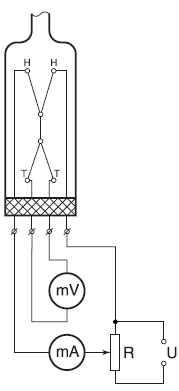
\includegraphics[height=45mm]{pic3.png}
		\caption{Схема термопарного манометра с лампой ЛТ-2 \label{overflow}}
	\end{figure}	
	\begin{figure}[h!]
		\centering
		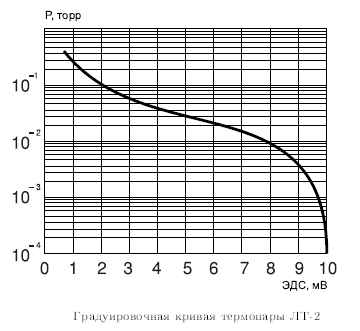
\includegraphics[width=45mm]{pic4.png}
		\caption{Градуировочная кривая термпопары ЛТ-2 \label{overflow}}
	\end{figure}
	\begin{figure}[h!]
		\centering
		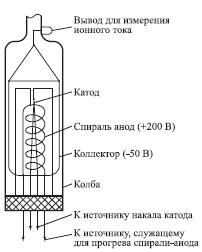
\includegraphics[width=45mm]{pic5.png}
		\caption{Схема ионизационной лампы ЛМ-2 \label{overflow}}
	\end{figure}
	
	\newpage
	\section{Ход работы}
	\subsection{Определение объема форвакуумной и высоковакуумной частей установки}
	\begin{table}[h!]
 		\centering
    	\begin{tabular}{| c | c | c | c | c |}
    		\hline
    		
    		V\textsubscript{К\textsubscript{5}+
    		                К\textsubscript{6}+кап, 
    		                см\textsuperscript{3}} & 
    		                
    		L\textsubscript{кап}, мм &
    		d\textsubscript{кап}, мм &
    		P\textsubscript{0}, Па$*$10\textsuperscript{3} &
    		%$\rho$%
    		$\rho\textsubscript{масла} \frac{\text{г}}{\text{см}^3}$ \\
    		\hline
    		40$\pm$2 & 75 & 1,22 & 102,4 & 0,885 \\
    		\hline
    	\end{tabular}
  		\caption{Данные установки}
	\end{table}
	Закроем краны К\textsubscript{5} и К\textsubscript{6}, в этих кранах и соединяющем их капилляре "запирается" (40$\pm$2)см\textsuperscript{3} воздуха. 
	Закроем краны К\textsubscript{1} и К\textsubscript{2}, включим форвакуумный насос и откачаем воздух до $10^{-2}$ торр. Перекрытием крана К\textsuperscript{3} отсоединим высоковакуумную часть от форвакуумной. Закрыв кран К\textsubscript{4}, приведем масляный манометр в готовность. Откроем, выпустив запертый воздух, кран К\textsubscript{5}. Измерим изменение давления в установке (откачали до $p=7\cdot10^{-3}$ мм.рт.ст. при $I=128$ мА).
	\begin{equation}
		\Delta h_\text{ф.в.}=h_1-h_2=(30,9-21,5)=9,40 \text{ мм}
	\end{equation}
	Закон Бойля-Мариотта:
	\begin{equation}
		V_\text{ф.в.}\approx\frac{P_0V\text{\textsubscript{К\textsubscript{5}+
    		                К\textsubscript{6}+кап, 
    		                см\textsuperscript{3}}}}{\rho g\Delta h}=0,05 \text{ м}^3
	\end{equation}
	\begin{equation}
	\sigma V=V*\sqrt{0,0025+0,0028}=0,05V=0,0026\text{ м}^3
	\end{equation}
	\begin{equation}
	V_\text{ф.в.}=0,05+0,0026 \text{ м}^3
	\end{equation}
	Откроем, чтобы газ распротранился на всю установку:
	\begin{equation}
	\Delta h=29,5-23,1 \text{ мм}=6,4 \text{ мм} 
	\end{equation}
	\begin{equation}
	V_\text{в.в}\approx \frac{P_0V_{K_5+K_6+kap}}{P_2}-V_\text{ф.в.}\approx\frac{P_0V_{K_5+K_6+kap}}{\rho g \Delta h_2}-V_\text{ф.в.}=0,02 \text{ м}^3
	\end{equation}
	\begin{equation}
	\sigma_V=0,001 \text{ м}^3
	\end{equation}
	\begin{equation}
	V_\text{в.в.}=0,020+0,001 \text{ м}^3
	\end{equation}
	
	\subsection{Получение высокого вакуума}
	Откачаем установку форвакуумным насосом. После того, как давление упало ниже $3\cdot 10^{-2} торр$, закроем кран и начнем высоковакуумную откачку. Включим ионизационный манометр. Измерим предельное давление в системе:
	\begin{equation}
	P_\text{пр}=(2,1 \pm 0,1) \cdot 10^{-4} \text{ торр}
	\end{equation}
	\begin{table}[h!]
 		\centering
    	\begin{tabular}{|c|c|c|c|c|c|c|c|c|c|c|c|}
    		\hline
    		t, c & 0,8 & 1,3 & 2,8 & 4,4 & 5,95 & 9,15 & 12 & 15,8 & 22 & 32,7 \\
    		\hline
    		P, $10^{-4}$ торр & 10 & 9,1 & 8,2 & 7,0 & 5,9 & 5 & 4,4 & 3,9 & 3,5 & 3,0 \\
    		\hline
    		$ln(P-P_\text{пр})$ & -7,14 & -7,26 & -7,4 & -7,62 & -7,87 & -8,14 & -8,37 & -8,62 & -8,87 & -9,32 \\
    		\hline
    	\end{tabular}
  		\caption{Изменение показаний показаний ионизационного манометра во времени при улучшении вакуума}
	\end{table}
	\begin{equation}
	ln(P-P_\text{пр})=-\frac{W}{V}t+lnP_0 \rightarrow W=\frac{lnP_0-ln(P-P_\text{пр})}{t}V=8,7\cdot 10^-2 \text{ }\frac{\text{л}}{\text{с}}
	\end{equation}
	\begin{equation}
	\sigma _W=1,1 \cdot 10^{-2} \text{ } \frac{\text{л}}{\text{с}} \rightarrow W=(8,7\pm 1,1) \cdot * 10^{-2} \frac{\text{л}}{\text{с}}
	\end{equation}
	Оценим величину потока. Для этого перекроем и отметим изменение показаний ионизационного манометра во времени:
	
	\begin{table}[h!]
 		\centering
    	\begin{tabular}{|c|c|c|c|c|c|c|c|c|c|}
    		\hline
    		t, c & 0 & 4,65 & 16,35 & 28,95 & 44,5 & 59,1 & 73,5 & 97 \\
    		\hline
    		P, $10^{-4}$ торр & 2,5 & 3 & 4 & 5,1 & 6,3 & 7 & 8,5 & 9,5\\
    		\hline
    	\end{tabular}
  		\caption{Изменение показаний показаний ионизационного манометра во времени при ухудшении вакуума [$k=(0,068\pm 0,003)\cdot 10^{-4} \frac{\text{торр}}{\text{с}}]$}
	\end{table}
	Мы знаем, что в данном случае (без откачки) изменение давления во времени описывается уравнением:
	\begin{equation}
	V_\text{вв}dP=(Q_\text{д}+Q_\text{и})dt \rightarrow Q_\text{д}+Q_\text{и} = kV_\text{вв}
	\end{equation}
	Также
	\begin{equation}
	Q_\text{н}=P_\text{пр}W-Q_\text{д}-Q_\text{и}
	\end{equation}
	Тогда:
	\begin{equation}
	Q_\text{н}=P_\text{пр}W-kV_\text{вв}=(1,69\pm 0,4)\cdot 10^{-4} \text{ кг}\cdot \frac{\text{м}}{\text{с}}
	\end{equation}
	Откроем К\textsubscript{6}, создадим таким образом исскуственную течь. Измерим установившееся давление P\textsubscript{уст}.
	\begin{equation}
	P_\text{уст}=2,6\cdot 10^{-4} \text{ торр}
	\end{equation}
	Рассчитаем производительность насоса по различию P\textsubscript{уст} и P\textsubscript{пр}. Для этого используем формулу течения газа через трубу, получим из нее $\frac{d(PV)}{dt}$ для капилляра.
	\begin{equation}
	\frac{d(PV)}{dt}=\frac{4}{3}r^3\sqrt{\frac{2\pi RT}{\mu}}\frac{P_\text{фв}-P_\text{уст}}{L}
	\end{equation}
	Стационарное состояние установки без течи (P=P\textsubscript{пр}):
	\begin{equation}
	P_\text{пр}W=Q\text{, [Q - воздухопотери]}
	\end{equation}
	Стационарное состояние установки с течью (P=P\textsubscript{уст}):
	\begin{equation}
	P_\text{уст}W=Q+\left(\frac{d(PV)}{dt}\right)_\text{капилл}=P_\text{пр}+\frac{4}{3}r^3\sqrt{\frac{2\pi RT}{\mu}}\frac{P_\text{фв}-P_\text{уст}}{L}
	\end{equation}
	Откуда:
	\begin{equation}
	W=\frac{4}{3}r^3\sqrt{\frac{2\pi RT}{\mu}}\frac{P_\text{фв}-P_\text{уст}}{L(P_\text{уст}-P_{пр}}=(9,9\pm 0,9)\cdot 10^{-2} \text{ } \frac{\text{л}}{\text{с}}
	\end{equation}
	Учитывая погрешность, можно считать, что результат совпал с ранее вычисленным значением.
	\newpage
	\section{Графики}
	\begin{figure}[ht!]
		\centering
		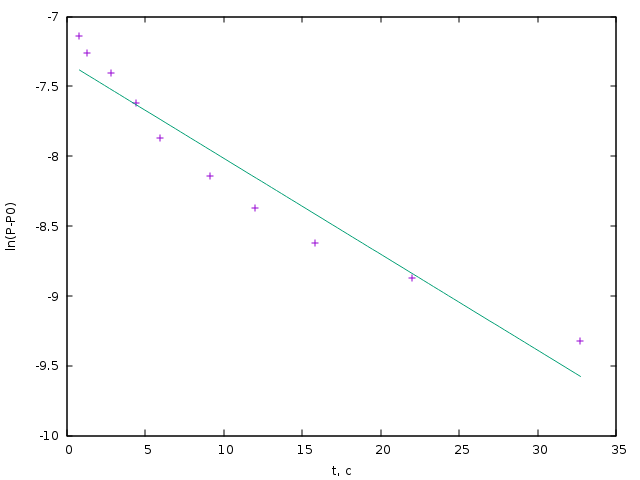
\includegraphics[width=100mm]{graph1.png}
		\caption{Изменение показаний показаний ионизационного манометра во времени при улучшении вакуума\label{overflow}}
	\end{figure}
	\begin{figure}[ht!]
		\centering
		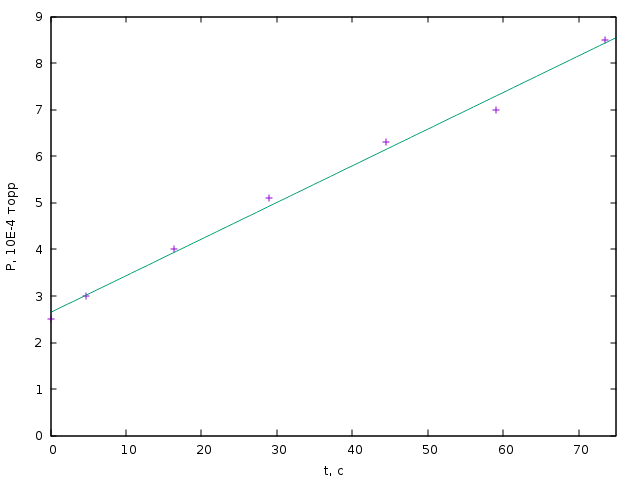
\includegraphics[width=100mm]{graph2.png}
		\caption{Изменение показаний показаний ионизационного манометра во времени при ухудшении вакуума\label{overflow}}
	\end{figure}
\end{document}
